% -*- mode: LaTeX; tex-main-file: "../Notes.tex"; -*-
\section{Background: Musical Signals}
\subsection{Mathematics of the Pure Tone}
The pure tone is the most elementary of all signals
(Hartmann~\cite{Hartmann:1998}).  Mathematically it is known as the
sine wave, a function of time described by the equation 
\begin{equation}
\label{eqn:puretone}
x(t) = A \sin(2 \pi t/T + \phi)
\end{equation}
where $A$ is the \emph{amplitude}, $T$ is the \emph{period} in
seconds, and $\phi$ is the \emph{phase} in radians.  The units of $x$,
whatever they might be (mechanical displacement, pressure, voltage),
are the same as the units of the amplitude $A$.

The sine function is periodic; it repeats itself when its argument,
the \emph{instantaneous phase} $2\pi t/T + \phi$, changes by $2\pi$.
Equation~(\ref{eqn:puretone}) shows that if $t$ starts at $t_0$ and
increases to $t_0 + T$, the function comes back to its starting
point; that is,
\[x(t_0) = x(t_0 + T)\]
This is why $T$ is called the period, measured in units of seconds per
cycle.  Its inverse, measured in units of cycles per second (Hz) is
called the \emph{frequency} of the wave,
\[f = 1/T\]
Because there are $2 \pi$ radians in a cycle, the \emph{angular
frequency}, $\omega$, is related to the frequency by 
\[\omega = 2 \pi f\]
The angular frequency is measure in radians per second.  Therefore, one
can write the sine wave with respect to these alternative units of
frequency: 
\[
x(t) %= A \sin(2 \pi t/T + \phi) 
= A \sin(2 \pi ft + \phi) = A \sin(\omega t + \phi)
\]

Like any other periodic tone, the pure tone can be characterized by
the psychological dimensions of \emph{pitch, loudness,} and \emph{tone
color}.  The pure tone actually serves as a reference for pitch
because of the latter's relation to the physical quantity of
frequency.

The standard textbook range of audible frequencies is from 20 Hz to
20000 Hz (Hartmann \emph{op.~cit.}).  The upper limit
depends greatly on age and otological history.  For the majority of
young adults the upper limit is likely to be closer to 17,000 Hz.  The
lower limit of 20 Hz is also problematic.  In order to make a 20-Hz
tone audible one must use a strong signal, but this runs the risk of
creating harmonic distortion, particularly at the third harmonic (60
Hz), because the hearing organ is so much more sensitive at 60 than
at 20 Hz.

The term \emph{tone color} refers to that part of timbre that is
attributable to the steady state part of a tone; i.e., the tone
without transients associated with onset, offset, or ongoing
aperiodic fluctuations (Hartmann \emph{op.~cit.}).  A pure tone
with a frequency below 200 Hz is judged as ``dull,'' while a tone with
a frequency greater than 2000 Hz is ``bright.''  Most of the energy in
speech signals is below 2000 Hz, and although numerous medieval
woodwind instruments had spectra that extended to high frequencies,
most modern musical instruments act as low-pass filters that attenuate
harmonics with frequencies greater than 1000 Hz.  This is true of
strings, brass, and woodwind instruments.  There are exceptions -- the
piccolo, for example -- and there are organ pipes with fundamental
frequencies as high as 8372 Hz ($C_9$).

% (begin: insert file synthesis.tex)
\ifthenelse{\boolean{nofootnotes}}{\subsection{Analysis and Synthesis}}
{\subsection{Analysis and Synthesis\protect\footnotemark}
\footnotetext{The first half of this section is based on parts of
Sethares~\cite{Sethares:1997}, and Irizarry~\cite{Irizarry:1998}}}
\label{sec:synthesis}
Although it can produce a tone, an individual sine wave has little
musical value by itself.  However, combinations of sine waves can be
used to describe, analyze, and synthesize almost any possible sound.
A complex sound can be modeled as a function of time, $x(t)$.  It can
be decomposed into a family of simple sine waves, each of which is
characterized by its frequency, amplitude,  and phase.  These
individual waves are called the {\it partials} 
(or {\it overtones}) and the collection of all the partials is called
the {\it spectrum} of $x$.  If the overtones occur at integer
multiples of the lowest frequency (fundamental) wave, then the
overtones are sometimes called {\it harmonics}.

As a simple example, consider a sine wave with unit amplitude and a
frequency of 440 Hz -- so called ``concert A'', or $A_4$.  Then
introduce a second sine wave with amplitude 1.2 and frequency 220 Hz
(one \emph{octave} below the first).  These two waves are shown as (a)
and (b) in Figure~\ref{fig:synth1}.  When the waves are sounded
together, the amplitudes are added together point by point and the
result is the complex wave shown in (c) of the figure.  This example
illustrates the distinction between what is known as a ``pure tone,''
(a) and (b), and a ``complex tone,'' (c). 
\begin{figure}
\ifthenelse{\boolean{nofigures}}{}{
  %             \pdfimage
  %             width 120 mm %             width 13 cm
  %             height 70 mm %             height 10 cm
  %             {\HOME/figures/Synthesis1.png}
\centering
  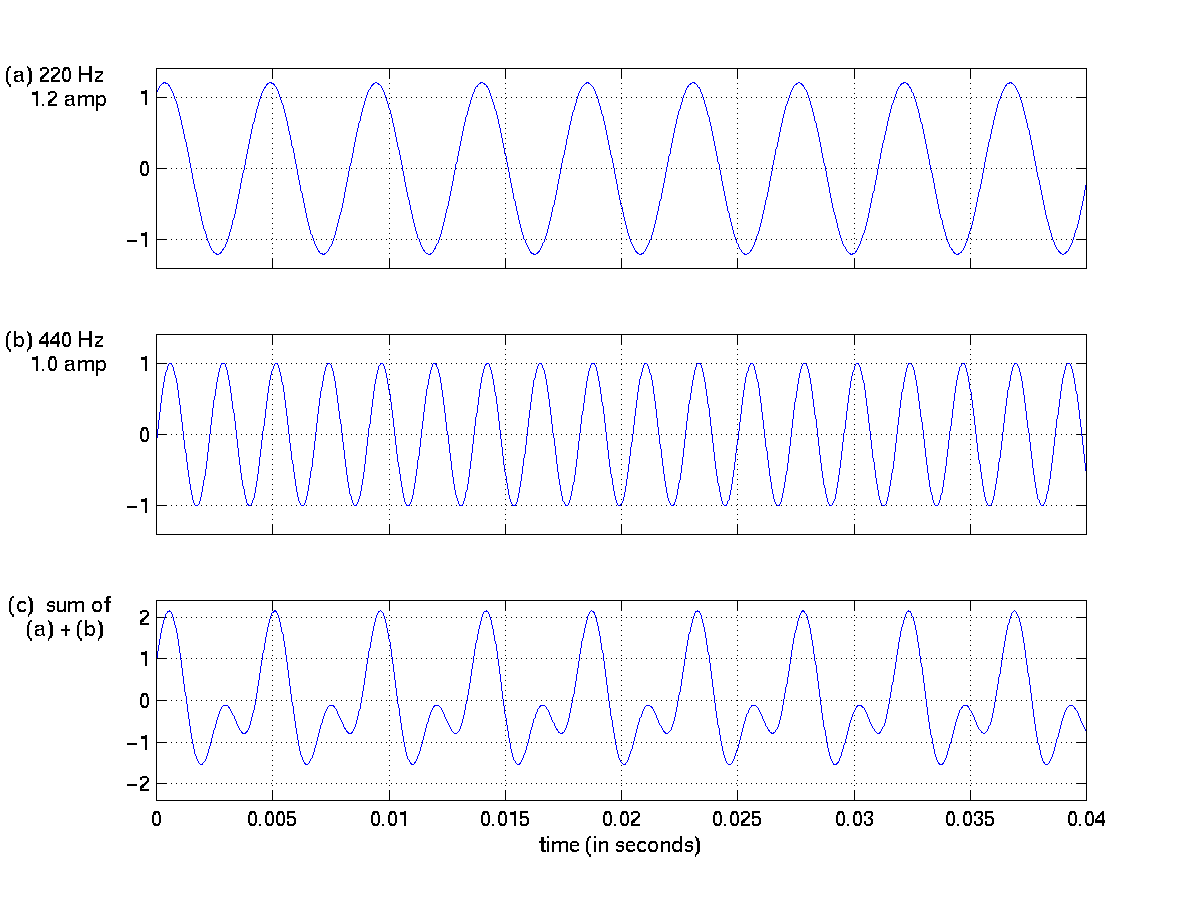
\includegraphics[width=120mm, height=70mm]{\HOME/figures/Synthesis1}
} % end ifthenelse
\caption{Synthesis by addition of two pure sine waves, (a)+(b)=(c).}
\label{fig:synth1}
\end{figure}

The technique of expressing a function as a sum of sinusoidal
components has been around for at least 200 years.  It is important
not only for our analytic understanding of sound waves, but also for
understanding the human perception of sounds.  It is believed that the 
ear functions as a kind of biological spectrum analyzer.  That is,
when sound waves impinge on the ear, what we perceive is a direct
result of the spectral components of the sound, and is only indirectly
a result of the composite waveform.

%% (begin: included from file phase.tex)
Take the wave forms in Figure~\ref{fig:synth1} for example.  Our eardrum
vibrates under the influence of the composite wave appearing in part (c).
However, the mechanisms of the inner ear -- our spectrum analyzer --
enable us to perceive the sound more precisely as a composition of (a)
and (b).  In Figure~\ref{fig:synth2}, sine wave (b) is still
modulating at 440 Hz, but it now begins at a different phase.
Therefore, the composite wave form shown in part (c) of
Figure~\ref{fig:synth2}, has a very different shape than that of
Figure~\ref{fig:synth1}. Yet the human ear perceives the same sound,
since both waves comprise the same frequency components.  
\begin{figure}
\ifthenelse{\boolean{nofigures}}{}{
%             \pdfimage
%             width 120 mm %             width 13 cm
%             height 70 mm %             height 10 cm
%             {\HOME/figures/Synthesis2.png}
\centering  
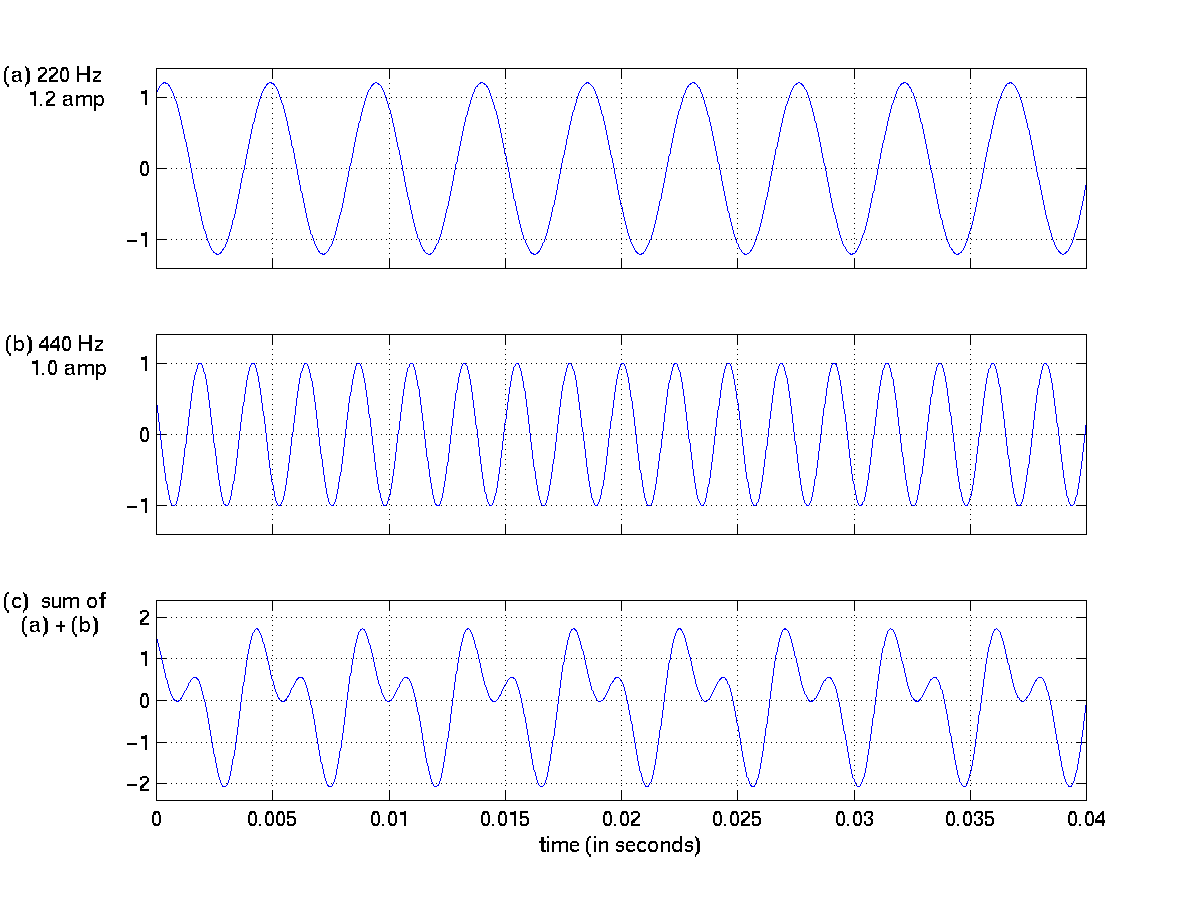
\includegraphics[width=120mm, height=70mm]{\HOME/figures/Synthesis2}
}
\caption{Synthesis by adding sine waves having the same frequencies as
those of Figure~\ref{fig:synth1}, but now the phase of sine wave (b) has
been shifted. Though waveform (c) looks different from that of
Figure~\ref{fig:synth1}, the same sound is perceived.}
\label{fig:synth2}
\end{figure}
%% (end: included from file phase.tex)

The foregoing presents a very basic idea underlying the formation of the
complex tone, $x(t)$.  It can be expressed mathematically as
\begin{equation}
\label{eqn:sumcos}
x(t) = \sum_{k=1}^K a_k \cos(\omega_k t + p_k)
\end{equation}
where the $a_k$ define the amplitudes associated with each partial and
the $p_k$ are some (usually arbitrarily specified) phases.  For
example, the figures above represent the function
\[x(t) = 1.2 \cos(220 t + p_1) + 1.0 \cos(440 t + p_2)\]
for $0 < t \leq (0.04)2\pi $ and $0 < p_k \leq 2\pi$.

The relevance of expression (\ref{eqn:sumcos}) for the analysis of
music is limited by the fact that real world signals, unlike those in
the figures, are never exactly periodic.  Strong similarities among
segments of signals often occur, which give rise to a sense of
pseudo-periodicity and, hence, pitch. However, superimposed on this
periodicity are fluctuations, noise, small frequency variations, etc.
These aperiodic components are due to different phenomena connected
with the particular physical mechanism used for the production of the
sound under analysis (Cavaliere and Piccialli).  For this reason, a
realistic model of a signal must generalize this simple,
time-invariant addition of periodic sine waves.  It should allow both
the amplitudes and frequencies to vary with time.  Writing 
$a_k = a_k(t)$ and $\omega_k t + p_k = \phi_k(t)$ accomplishes this
and yields the 
%following signal plus noise statistical model:
following sum of partials:
\begin{equation}
\label{eqn:sumpartials}
%y(t) = f[t|\beta(t)] + \epsilon(t), \mbox{ with }
x[t|\beta(t)] = \sum_{k=1}^K a_k(t) \cos(\phi_k(t))
\end{equation}
where the notation $x(\cdot|\beta)$ indicates that the
functional form of $x$ is conditional on the time-varying vector
$\beta(t) \equiv (a_1(t),\ldots,a_K(t),\phi_1(t),\ldots,\phi_K(t))^t$ of
amplitudes and phases.  This model also requires
that $a_k(t)$ and $\phi'_k(t)$ vary slowly~\cite{Rodet:1992}.  This
requirement as well as the relationship between the ``instantaneous
frequency,'' $\omega_k,$ and the time-varying phase, $\phi_k(t),$ will
be discussed in the following sections. 

Still implicit in model~(\ref{eqn:sumpartials}) is the assumption that
the signal is well approximated by a sum of pure sinusoidal waves.  
However, the presence of a given frequency, $\omega_k,$ can now be
short lived, and its contribution to $x$ varies (albeit slowly) with
time via $a_k(t)$.   
%Further, to account for the aperiodic component of the signal, a
%non-sinusoidal noise term, $\epsilon(t)$ appears.  The following
%sub-section describes the assumed functional form of $\epsilon(t)$ as
%well as
%As in Serra~\cite{Serra:1989}, we can take this to be a stationary
%autoregressive process.   

Assuming model (\ref{eqn:sumpartials}), the problem of analyzing a signal
becomes the estimation of $\beta(t),$ and there are as many approaches
to that problem as there are applications of signal analysis.  

In later sections, we consider which signal analysis methods are
particularly well suited to the type of musical analysis we wish to
perform.  Therefore, it is crucial that we have a good grasp of the
musical ideas underlying and motivating our research into musical
signal analysis.  The following section presents one such notion --
musical \emph{consonance}.  Also presented are some existing
quantitative measures of this concept. 
% (end: insert file synthesis.tex)

% (begin: insert file consonance.tex)
\subsection{Consonance and Dissonance}
\label{sec:consonance}
According to Tenney~\cite{Tenney:1988} and Sethares
\cite{Sethares:1997}, the historical usage of the term {\it
consonance} (and its antonym, {\it dissonance}) can be classified
according to five distinct categories.
(see~\cite{Sethares:1997} for more details)
\begin{enumerate}
\item {\bf Melodic Consonance (CDC-1)} successive melodic intervals are
consonance or dissonant depending on the surrounding melodic context;
refers to relatedness of pitches sounded successively (melodic contour)
\item {\bf Polyphonic Consonance (CDC-2)} consonance is a function of
the interval between (usually 2) simultaneously sounding tones;
proponents of this definition are clearest about the consonant
$\leftrightarrow$ ``pleasant'' association.
\item {\bf Contrapuntal Consonance (CDC-3)} consonance is defined by
its role in counterpoint, e.g.~voice-leading techniques; the 4th is
declared dissonant (in contrast to CDC-2).
\item {\bf Functional Consonance (CDC-4)} focus on relation of
individual tones to the root or tonic; consonant tones are those that
are in simple unison, third, or fifth relation to root.  Dissonance
occurs when the music moves away from root and sets up a desired
return; dissonances cause chordal motion (and not vice-versa);  Piston
in ``Harmony'' relates consonant with stable or complete
and dissonant with restless or requiring resolution; ``the
essential quality of dissonance is its sense of movement and
not...its degree of unpleasantness to the ear.''
\item {\bf Sensory Consonance (CDC-5)}  equates consonance with
smoothness and the absence of beats; equates dissonance with roughness
and the presence of beats.
\end{enumerate}

The definition of sensory consonance is based on the  phenomenon of
beats.  If two pure sine tones are sounded at almost the same
frequency, then beating occurs due to the interference between the
tones.  The beating becomes slower as the two frequencies approach
each other and disappears when they coincide.  Typically, slower  
beats are perceived as gentle and pleasant while fast beats are
perceived as rough and unpleasant. Observing that any sound can be
decomposed into sinusoidal partials, Helmholtz \cite{Helmholtz:1877}
theorized that the perception of dissonance in a musical tone is
determined by the presence and quality of beats among the tone's
interacting partials. 

The present research effort is directed at the discovery of a
definition that might reconcile these competing notions of consonance.
In particular, we  would like to exploit the theory of \emph{sensory}
and \emph{tonal} consonance (CDC-2 and CDC-5)
of Plomp and Levelt~\cite{Plomp:1965} as well as its elaboration
in~\cite{Sethares:1997}.  Some of this theory is described below in
section~\ref{sec:disscurves}.  Briefly, it employs functions called
\emph{dissonance curves} which measure the ``sensory'' dissonance, of
a complex tone at each particular instant in time.\footnote{Really, a
small interval of time is required to ascertain what (pseudo-)periodic
frequencies are present at a particular instant.}   
This provides a useful point-wise measure.
However, we would also like a measure that is dynamic and appeals to a
melodic sense of consonance.  For example, a dissonance curve does not
account for dissonance due to melodic changes from one complex tone to
the next.  

\subsection{Dissonance Curves}
\label{sec:disscurves}
Two pure sine waves are both perceptible if the frequencies are well
separated.  When the frequencies are close together, only one sine
wave is heard (though possibly with beats).  By varying the frequency
of one of the waves while keeping the other wave fixed, Plomp and
Levelt~\cite{Plomp:1965} gathered data revealing subject's preferences
for various frequency intervals.  An example of what these data
indicate appears as a \emph{dissonance curve} in 
Figure~\ref{fig:1DissCurve}.  (One method of deriving such curves in
practice is described in section~\ref{sec:FourierDissonance}.)  The
curves in the figure are in stark contrast to existing musical theory.
In particular they imply that, in terms of sensory dissonance,
intervals such as the major 7th and minor 9th are almost
indistinguishable from the octave.  This leads some to argue that
these data bear no relation to our notions of musical
consonance. Regardless of whether they have a direct influence on our
ideas about musical intervals, dissonance curves provide a way to
measure the intervals among \emph{pure sine waves}.  Therefore, they
can be useful when analyzing a musical signal that has been decomposed
into its spectral components.

\begin{figure}
\ifthenelse{\boolean{nofigures}}{}{
\centering  
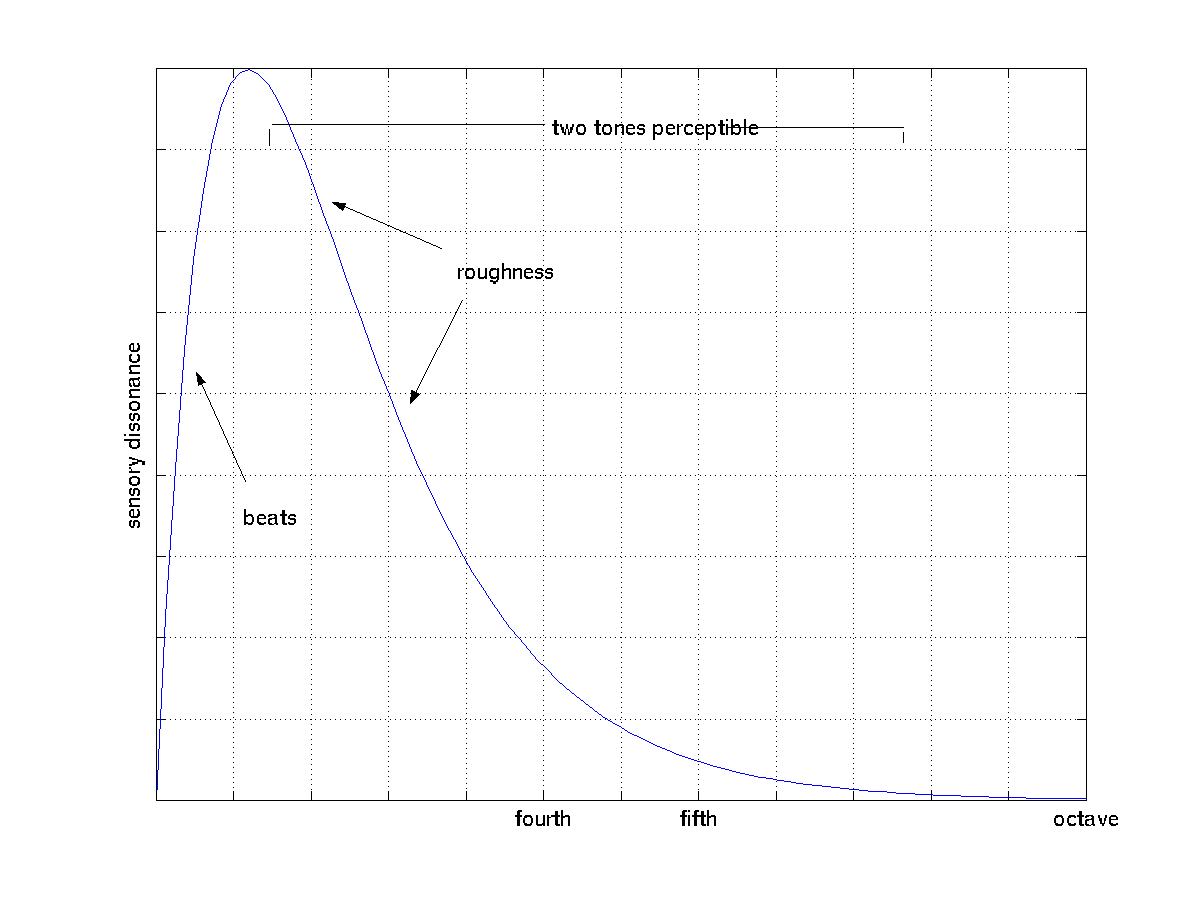
\includegraphics[width=120mm, height=70mm]{\HOME/figures/1DissCurve}
}
\caption{{\small Two sine waves are sounded simultaneously.  Typical
perceptions include pleasant beating (at small frequency ratios),
roughness (at middle ratios), and separation into two tones (at first
with roughness, and later without) for larger ratios.  the horizontal
axis represents the frequency interval between the two sine waves,
and the vertical axis is a normalized measure of ``sensory''
dissonance.  The frequency of the lower sine wave is 400 Hz}}
\label{fig:1DissCurve}
%\end{figure}
%\begin{figure}
\ifthenelse{\boolean{nofigures}}{}{
%             \pdfimage
%             width 120 mm 
%             height 70 mm
%             {\HOME/figures/3DissCurves.png}
\centering  
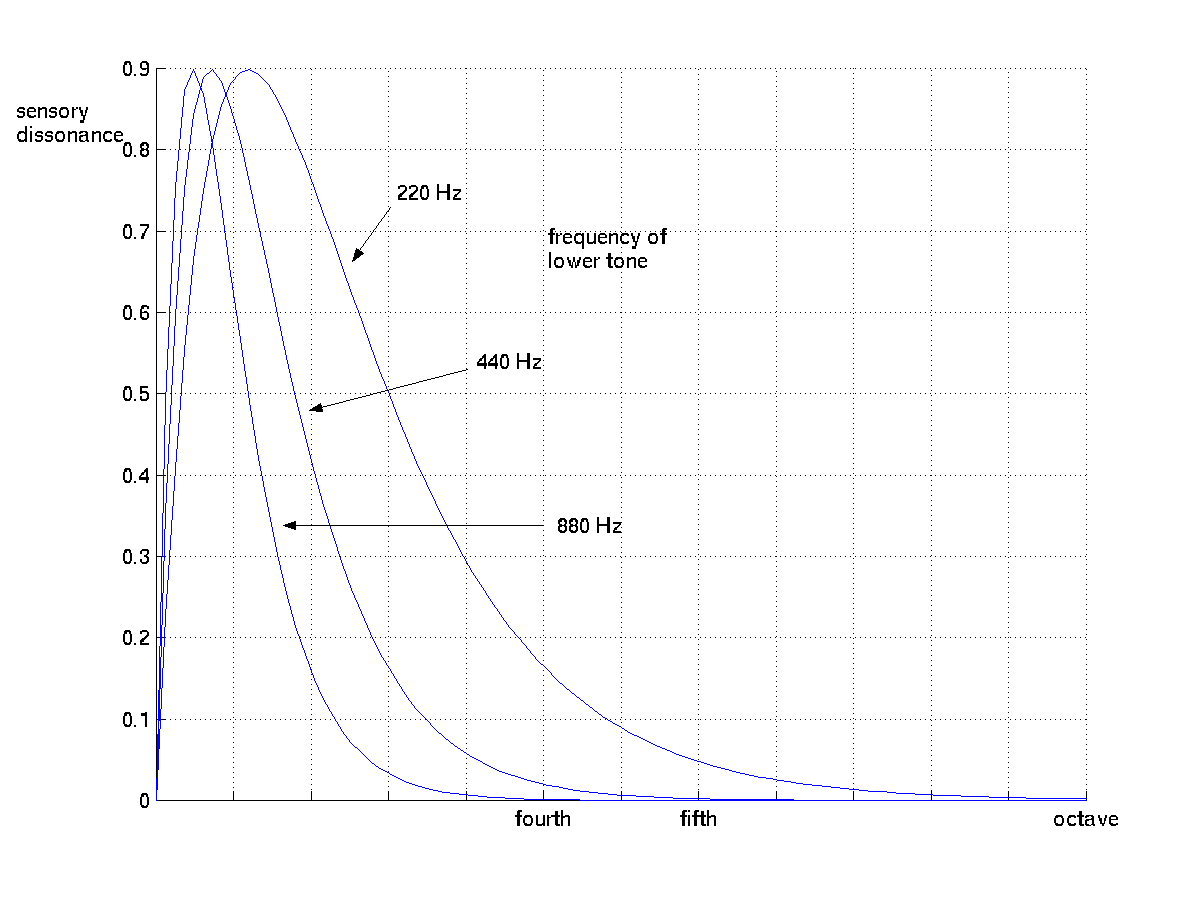
\includegraphics[width=120mm, height=70mm]{\HOME/figures/3DissCurves}
}
\caption{{\small Two sine waves are sounded simultaneously.  The
horizontal axis represents the frequency interval between the two sine
waves, and the vertical axis is a normalized measure of ``sensory''
dissonance. The plot shows how the sensory consonance and dissonance
change depending on the frequency of the lower tone.}}
\label{fig:3DissCurves}
\end{figure}
% (end: insert file consonance.tex)

%%% NEWER (UNDERDEVELOPED) IDEAS %%%
%Recall equation~(\ref{eqn:sumpartials}) of section~\ref{sec:synthesis}
%in which a complex tone $x$ is modeled as a weighted sum of sinusoidal
%partials: 
%\[x(t) = \sum_{k=1}^K a_k(t) \cos(\phi_k(t))\]
%where the instantaneous frequency of the $k$th partial is
%%(cf.~\S~\ref{sec:instfreq}, equation~\ref{eqn:sumpartials}): 
%\[\omega_k(t) = \phi'_k(t) \geq 0.\]
%Suppose for simplicity that the set of $K$ instantaneous frequencies
%$\{\omega_k\}$ are known and constant over a small interval (instant)
%of time.  Then...
%%the relative dissonances among the frequencies in a complex
%%tone
%
%It is possible that a particular \emph{instant} in a piece of music
%will have a high sensory dissonance value but, because of this
%instant's relation to its context, the section of the piece containing
%this instant has a low total dissonance value.  We can create measures
%that act in this way.  Consider a simple succession of 3 instants of a
%musical piece represented by $\{S_0, S_1, S_2\}.$  Let $\|\cdot\|$ be
%the measure of dissonance of $S_k.$  It is possible ...

